\begin{figure}[!ht]
    \centering
    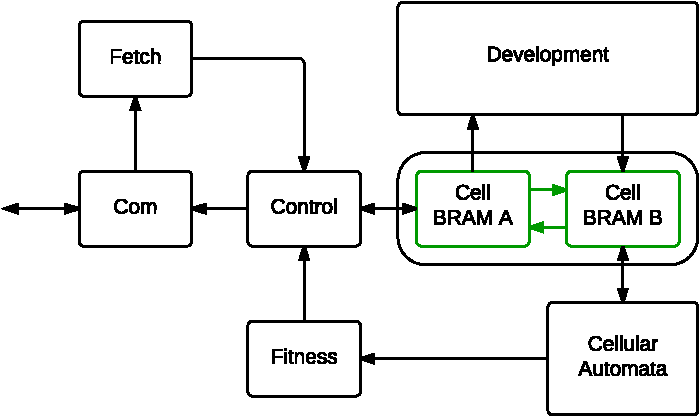
\includegraphics[width=0.8\textwidth]{implementation-simple}
    \caption{TODO}
    \label{fig:implementation-simple}
\end{figure}

\begin{figure}[!ht]
    \hspace{-0.1\textwidth}
    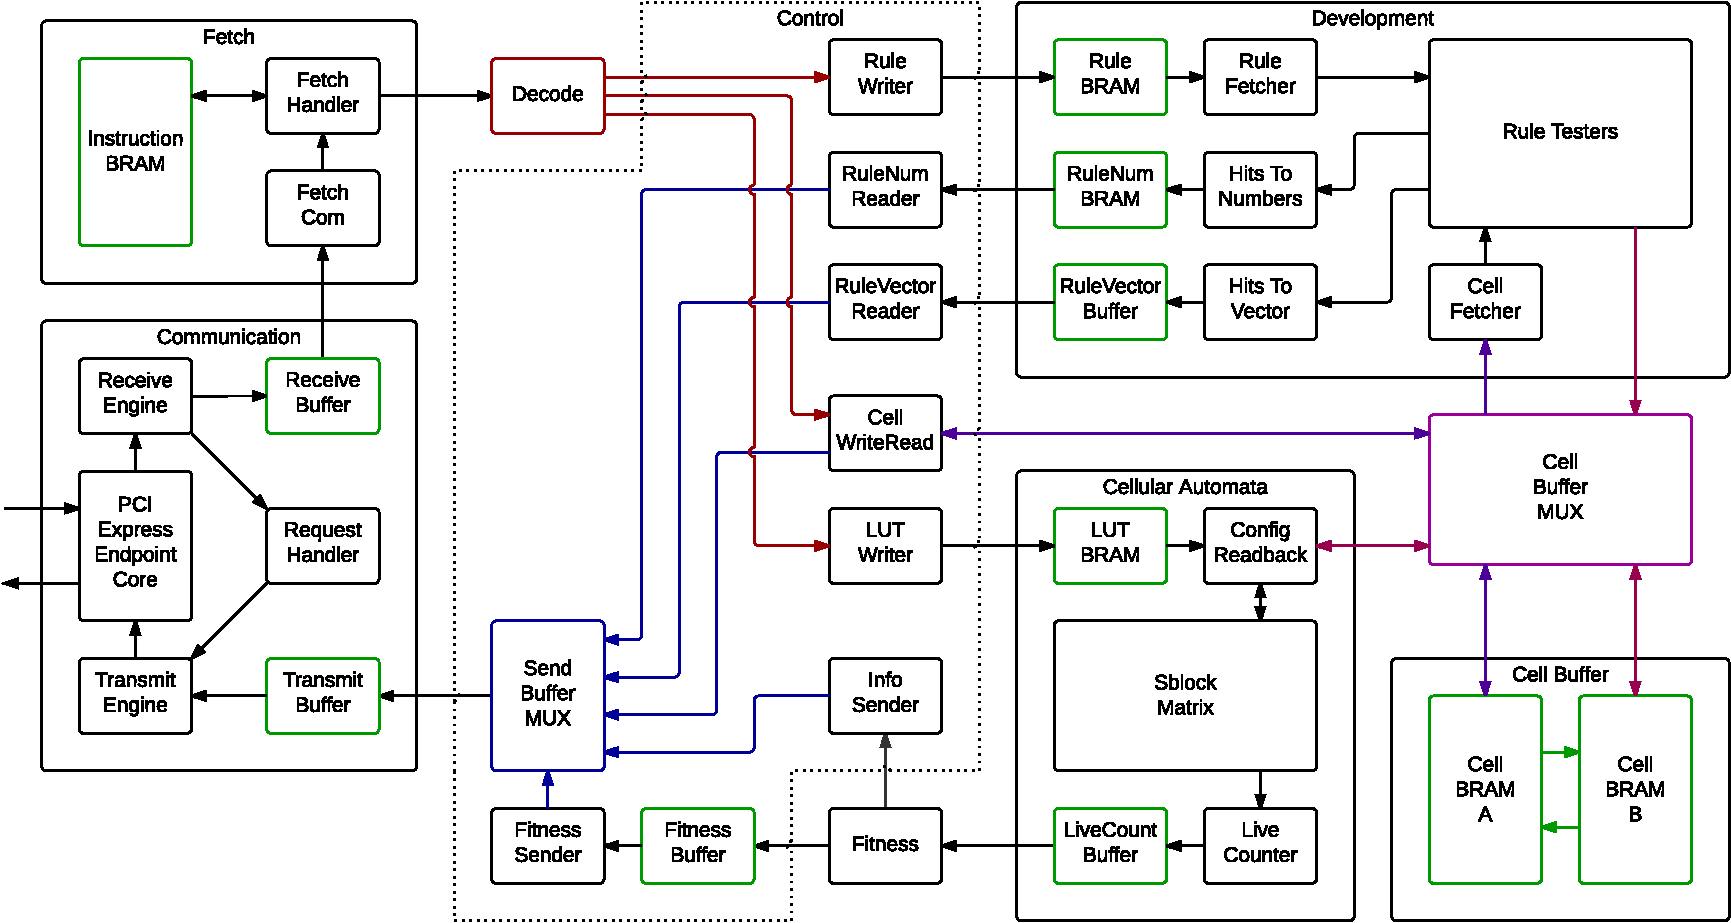
\includegraphics[width=1.2\textwidth]{implementation-full}
    \caption{TODO}
    \label{fig:implementation-full}
\end{figure}

The platform is design as an interlocked pipeline.
The main stages are Fetch, Decode and Execute, but due to interlocking, each stage can contain sub-pipelines or state machines.

The Execute stage is special in that is is split into many sub-modules, where only one is activated at a time.
The exception is Fitness, which is always active, since it operates in a dataflow-like fashion.
A hazard detection unit could be implemented to increase performance by allowing multiple non-conflicting units run in parallell.

Interlocking is implmented using special Run and Done signals.
Run is asserted when all modules asserts Done.

\section{Communication}

See previous report!

\section{Fetch}

Fetch is responsible for fetching the next instruction from either communication or internal memory.
It is also responsible for handling all control flow.

It has three modes of operation: FetchCom, FetchMem and StoreMem.

In FetchCom mode, instructions are fetched from communication and sent to decode.
Since a variable-length format is used, this may take multiple cycles.
To make sure that instructions in the pipeline completes, NOPs are sent when the receive buffer is empty.
When encountering a Store instruction, it enters StoreMem mode and for a Jump instructions it enters FetchMem mode.

In FetchMem mode, instructions are fetched from InstructionBRAM and sent to decode.
The first InstructionBRAM address is specified by the Jump instruction, and then it is incremented by one after each instruction.
When encountering a Break instruction, it enters FetchCom mode.

In StoreMem mode, instructions are fetched from communication and stored in InstructionBRAM.
The first InstructionBRAM address is specified by the Store instruction, and then it is incremented by one after each instruction.
Instructions are stored in full 256-bit format.
When encountering an End instruction, it enters FetchCom mode.

Control flow is implemented by having N M-bit general counters and a JumpEqual instruction.
The counters can be incremented or reset using special instructions.
The JumpEqual instruction is treated as a Jump instruction when the specified counter matches the specified value, otherwise it is discarded.

\section{Decode}

Decode is responsible for parsing instructions, setting control signals and passing instruction parameters to activated modules.

The control signals determine which module is activated, which modules the CellBufferMux and SendBufferMux will connect to, and if the CellBuffer should swap contents.

%\section{RuleWriter}

%RuleWriter is responsible for writing development rules to RuleBRAM.

%The instruction parameter is simply stored to the BRAM.

%\section{RuleNumberReader}

%RuleNumberReader is responsible for transferring rule numbers from the RuleNumberBRAM to the SendBuffer.

%As many rule numbers as can fit 32 bits are sent each cycle, but it is aligned for each row.

%\section{LUTWriter}

%LUTWriter is responsible for writing a LUT entry to LUTBRAM.

%The instruction parameter is simply stored to the BRAM.

\section{Cellular Automata}

The Cellular Automata module is responsible for configuring the sblock matrix with data from the Cell Buffer, step the sblocks and store the number of live cells, and read the new states back into the Cell Buffer.

It is implemented as a state machine that is manipulating a matrix of sblocks connected to an adder tree.
The adder tree is used to calculate the number of live cells after each step.
The numbers are then stored in the Live Count Buffer.
If the Live Count Buffer is full, data is overwritten, possibly corrupting fitness evaluation, until the buffers are reset.
This design decision was made to allow the CA to run without being required to read fitness data.

When configuring the sblock matrix, cell types are used as an index for the LUTBRAM to find the corresponding LUT entry.

\section{Development}

Development is responsible for reading the cells in cell BRAM A, change them based on development rules specified by the user, and write the result to cell BRAM B.

It is implemented as a state machine controlling an interlocked two-stage pipeline.

The first stage is CellFetch, which reads the cell neighborhoods for one row of cells per run.
\todo{explain access pattern}
This takes 3 cycles for 2D and 5 for 3D.

The second stage is implemented as yet another pipeline.
First, rules are fetched from RuleBRAM, then rules and cell neighborhoods are sent to the RuleTesters.
To allow multiple rules to be tested each cycle, RuleTesters is split into two parts.
The first part tests the different rules against each cell, while the second selects the result from the highest priority rule.
After the first part, hits are output from RuleTesters to HitsToVector and HitsToNumbers.
Finally, everything is stored to memory.
\footnote{Rule vectors are only stored after the final rules and cells}

The number of active rules can be set at runtime to reduce development time by skipping unused rules.
\TODO
\todo{CellFetch limiting factor for very few rules}
\todo{vectors overwritten to allow development without reading them}

\begin{itemize}
    \item Rule 0 reserved.
    \item Two-stag pipeline:
    \begin{itemize}
        \item CellFetch
        \item RuleFetch, Test, HitsToVec/Num, Write (4-stage pipeline)
    \end{itemize}
    \item Last triggered rules are written to RuleNumbersBRAM
    \item All triggered rules are written to RuleVectorBuffer (even overridden)
\end{itemize}

\section{Fitness}

\begin{itemize}
    \item Dataflow-ish (livecountbuffer to fitnessbuffer)
    \item Custom implementation, simple interface
    \item Example: LC, DFT
\end{itemize}

